\chapter{Grasping}
A three finger gripper configuration is assumed to be placed at the end effector of the Kuka iiwa arm. This gripper corresponds to the Barrett Hand, shown in Figure~\ref{fig:barrett_hand}.
\begin{center}
\begin{figure}[htbp]
\centering
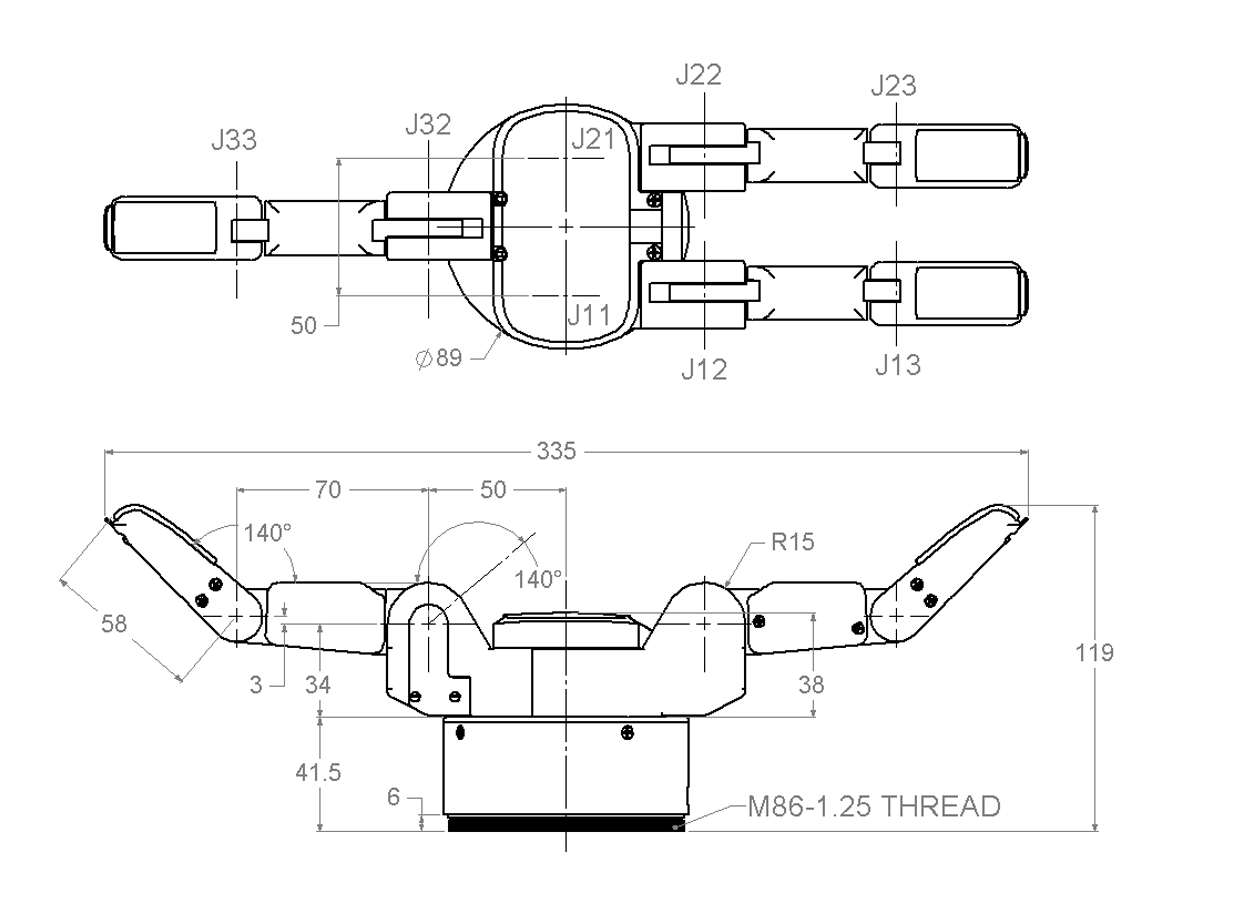
\includegraphics[width=0.8\textwidth]{images/bh8-282-dimensions.png}\\
\caption{Barrett Hand gripper (model BH8-282) dimensions}
\label{fig:barrett_hand}
\end{figure}
\end{center}
%
\section{Gripper \& Forward Kinematics}
The dimensions and angle parameters of each finger of this hand appear in Figure~\ref{fig:hand_dimensions} and the following three tables.
\begin{center}
\begin{figure}[htbp]
\centering
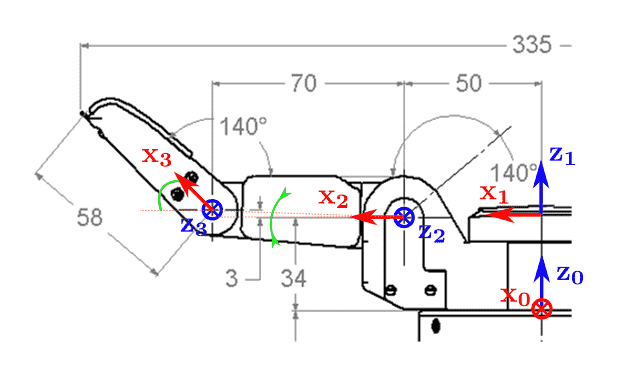
\includegraphics[width=0.8\textwidth]{images/bh8-282-generalized-finger-fwd-kin.png}\\
\caption{Coordinates systems for a generalized finger of the gripper}
\label{fig:hand_dimensions}
\end{figure}
\end{center}

\begin{center}
\begin{tabular}{ |c|c|c|c|c| } 
\hline
$i$ & $θ_i$ (rad) & $L_{i-1}$ (m) & $d_i$ (m) & $α_{i-1}$ (rad) \\
\hline
1 (J11) & $θ_{11} - π/2$ & 0.025 & 0.0034 & 0 \\
2 (J12) & $θ_{12} + 0.04$ & 0.05 & 0 & $π/2$ \\
3 (J13) & $θ_{13} + 0.69$ & 0.07 & 0 & 0 \\
\hline
\end{tabular}
\end{center}

\begin{center}
\begin{tabular}{ |c|c|c|c|c| } 
\hline
$i$ & $θ_i$ (rad) & $L_{i-1}$ (m) & $d_i$ (m) & $α_{i-1}$ (rad) \\
\hline
1 (J21) & $θ_{21} - π/2$ & 0.025 & 0.0034 & 0 \\
2 (J22) & $θ_{22} + 0.04$ & 0.05 & 0 & $π/2$ \\
3 (J23) & $θ_{23} + 0.69$ & 0.07 & 0 & 0 \\
\hline
\end{tabular}
\end{center}

\begin{center}
\begin{tabular}{ |c|c|c|c|c| } 
\hline
$i$ & $θ_i$ (rad) & $L_{i-1}$ (m) & $d_i$ (m) & $α_{i-1}$ (rad) \\
\hline
1 & $π/2$ & 0 & 0.0034 & 0 \\
2 (J32) & $θ_{32} + 0.04$ & 0.05 & 0 & $π/2$ \\
3 (J33) & $θ_{33} + 0.69$ & 0.07 & 0 & 0 \\
\hline
\end{tabular}
\end{center}

\section{Gripper Inverse Kinematics}

The following IK analysis referes to one finger of the Barrett Hand gripper, which has 3 revolute joints. Finger 3 has only 2 revolute joints for which the angle solutions are the same with the solutions of the last 2 joints of the other fingers. 

\begin{center}
\begin{figure}[!htb]
\centering
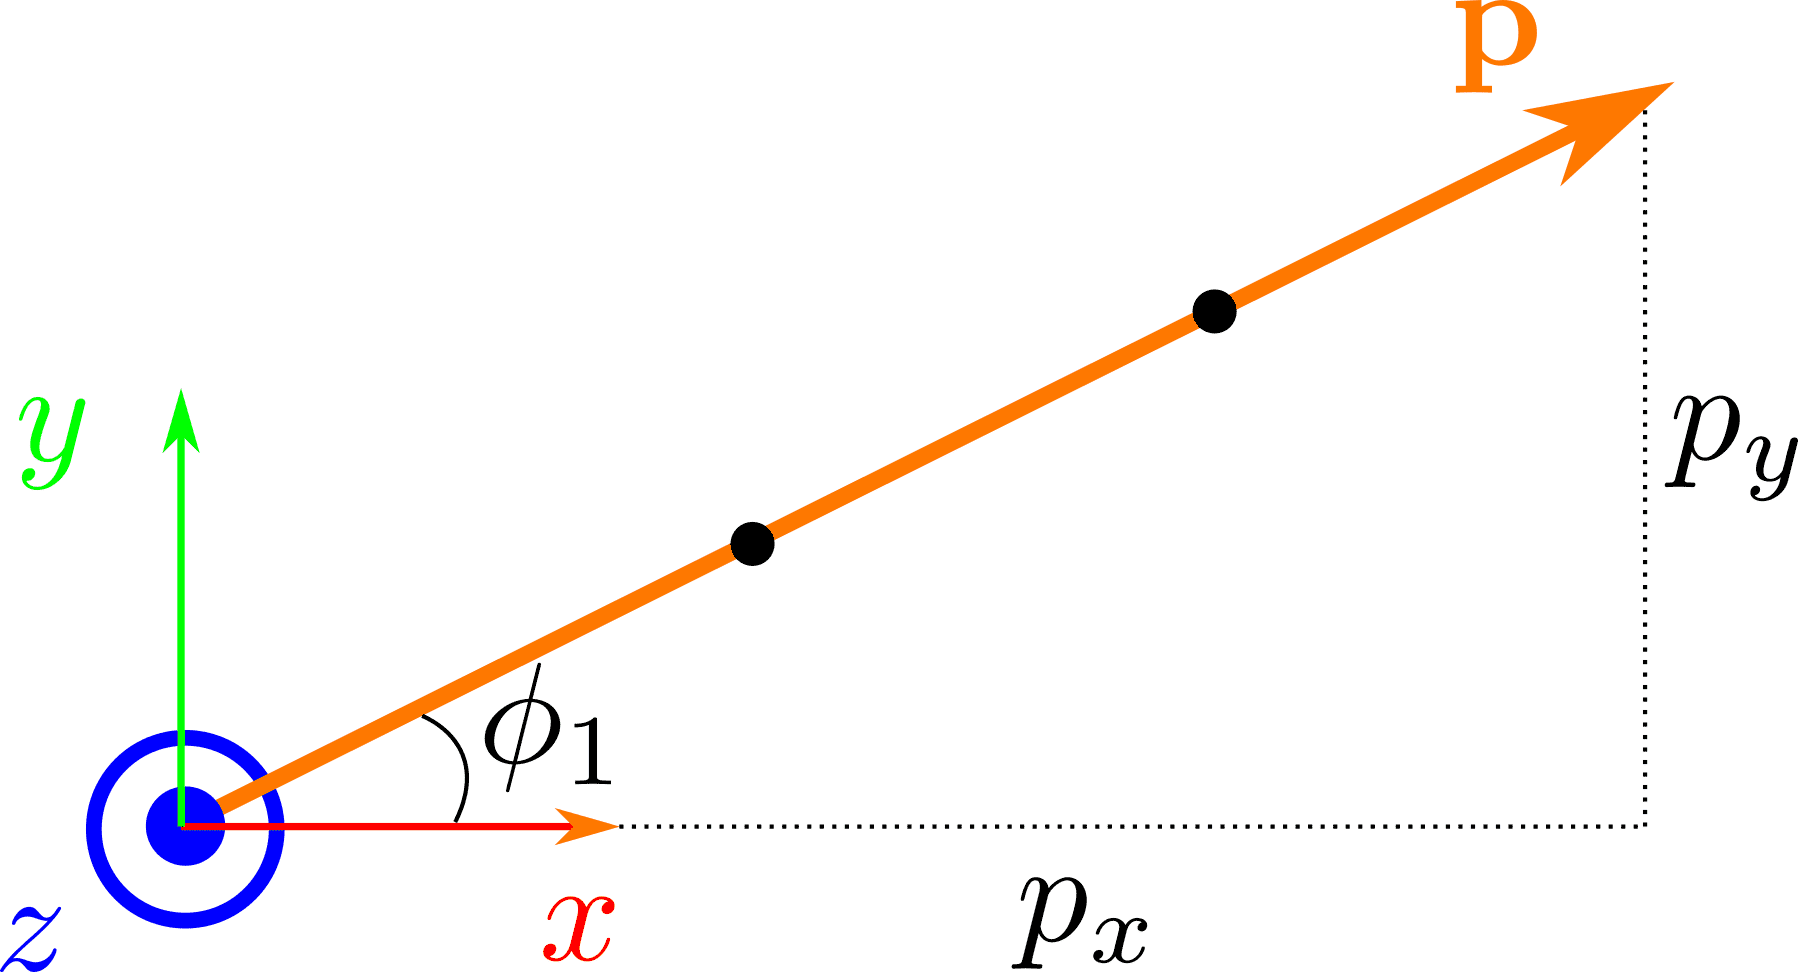
\includegraphics[width=0.5\textwidth]{images/grasper-rrr-top.png}\\
\caption{Top view of single finger of the gripper with 3 joints (RRR kinematic chain)}
\label{grasper-rrr-top}
\end{figure}
\end{center}

Let 
$
\mathbf{p} = \left[p_x, p_y, p_z \right]^T
$
be the position of the grasp point for one finger. The first angle can easily be calculated using the top view of Figure~\ref{grasper-rrr-top} from $φ_1 = atan2 \left( p_y, p_x \right)$
\begin{center}
\begin{figure}[htbp]
\centering
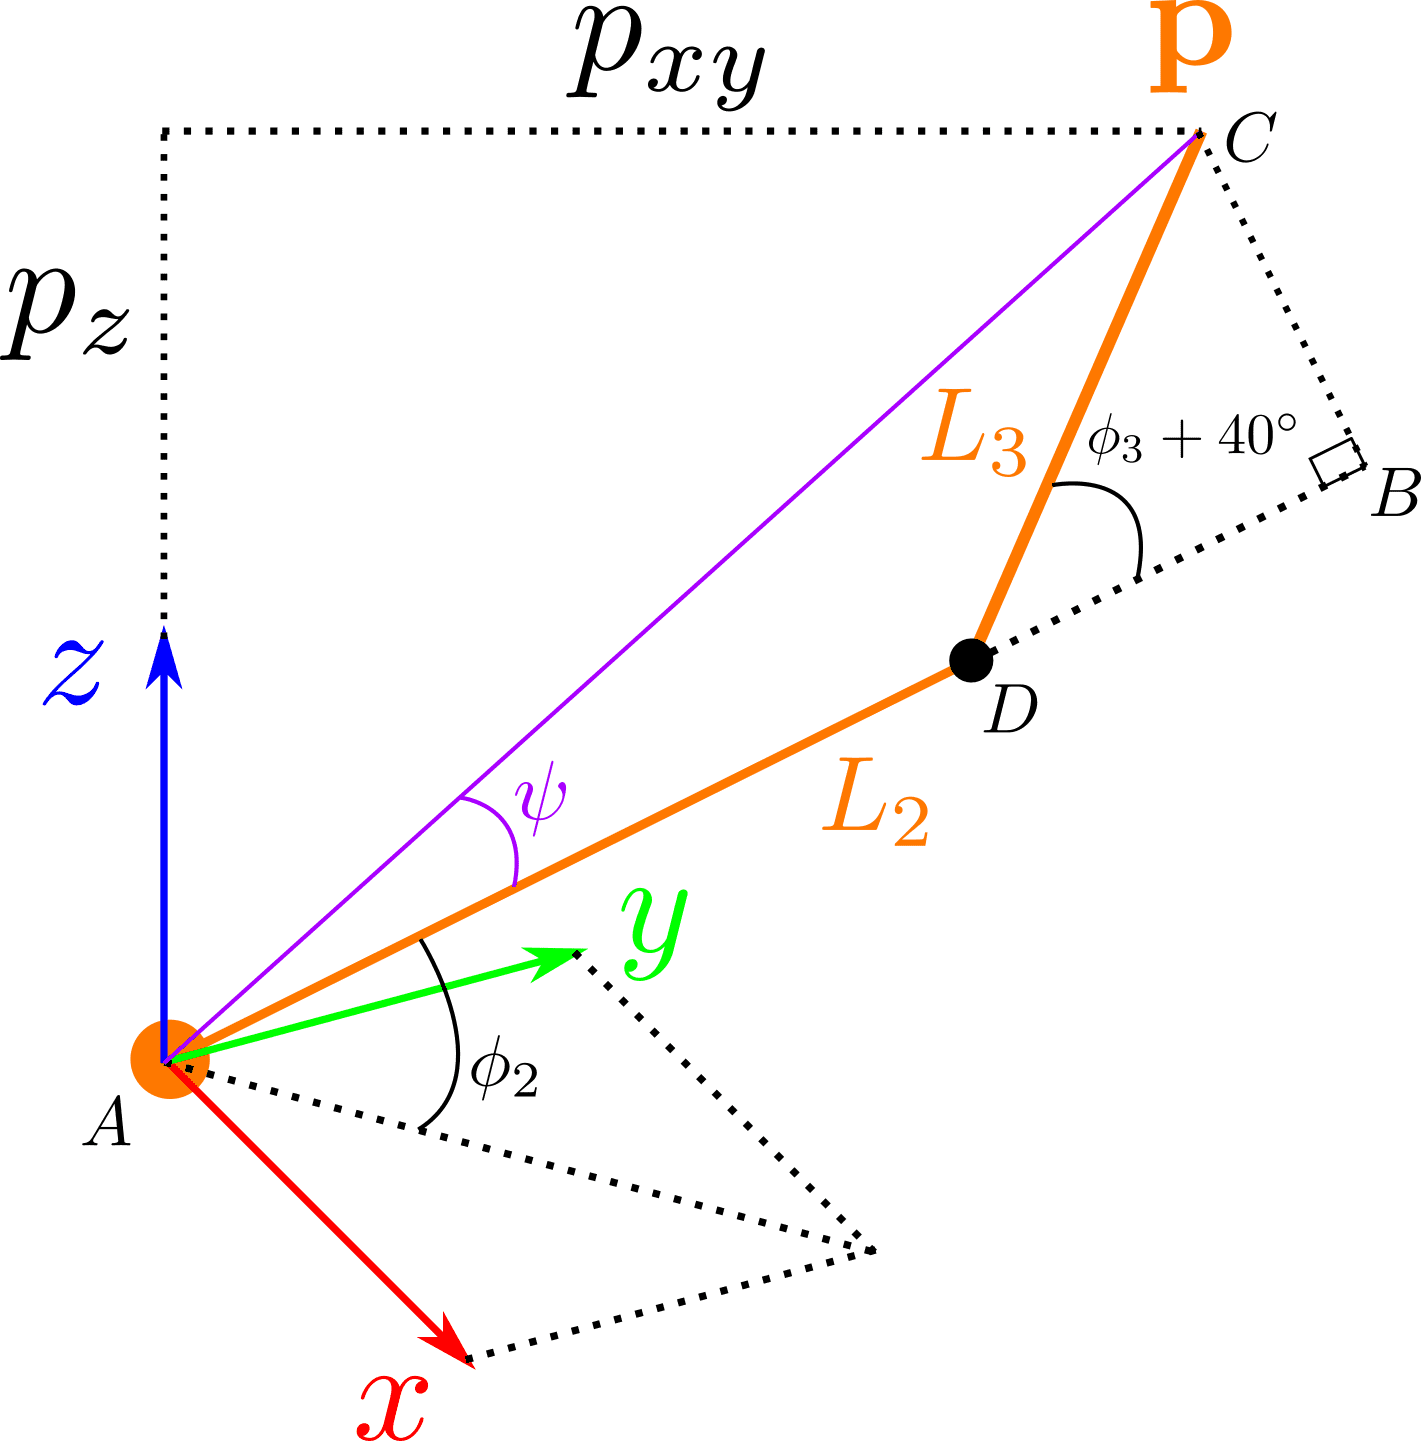
\includegraphics[width=0.5\textwidth]{images/grasper-rrr-side.png}\\
\caption{Side view of single finger of the gripper with 3 joints (RRR kinematic chain)}
\label{grasper-rrr-side}
\end{figure}
\end{center}

Geometric inspection of the noted quantities in Figure~\ref{grasper-rrr-side} provides
\begin{equation}
BD = L_3 \cos \left(φ_3 + \frac{2π}{9} \right)
,~
BC = L_3 \sin \left(φ_3 + \frac{2π}{9} \right)
,~
p_{xy} = \sqrt{p_x^2 + p_y^2}
\end{equation}

Next, we calculate the third angle based on the law of cosines applied on the triangle $ACD$ (see Figure~\ref{grasper-rrr-side})
\begin{equation}
\cos \left( π - φ_3 - \frac{2π}{9} \right) = \frac{L_2^2 + L_3^2 - p^2}{2 L_2 L_3}
,~
\cos \left(φ_3 + \frac{2π}{9} \right) = \frac{p^2 - L_2^2 - L_3^2}{2 L_2 L_3}
\end{equation}
\begin{equation}
φ_3 = atan2 \left[ \pm \sqrt{1 - \left( \frac{p^2 - L_2^2 - L_3^2}{2 L_2 L_3} \right)^2} , \frac{p^2 - L_2^2 - L_3^2}{2 L_2 L_3} \right] - \frac{2π}{9}
\end{equation}

In a more general case, the first argument of the $atan2$ function in the expression of $φ_3$ could also be negative,
but in this case this second solution is rejected, because due to mechanical constraints, this angle can not be negative. 
Having calculated $φ_3$ we calculate $φ_2 $

\begin{equation}
tan \left( ψ + φ_2 \right) = \frac{p_z}{\sqrt{p_x^2 + p_y^2}}
\end{equation}
\begin{equation}
ψ + φ_2 = atan2 \left( p_z, \sqrt{p_x^2 + p_y^2} \right)
\end{equation}
\begin{equation}
tan \left( ψ \right) = \frac{L_3 \sin \left( φ_3 + \frac{π}{4} \right) }{L_2 + L_3 \cos \left( φ_3 + \frac{π}{4} \right)}
\end{equation}
\small
\begin{equation}
φ_2 = atan2 \left( pz, \sqrt{p_x^2 + p_y^2} \right) - atan2 \left[ L_3 \sin \left( φ_3 + \frac{2π}{9} \right), L_2 + L_3 \cos \left( φ_3 + \frac{2π}{9} \right) \right]
\end{equation}
\normalsize

\section{Force closure}

In order to achieve a firm grasp of the surgical tool, the gripper fingers must be positioned in such a way around the object so that there is \textbf{force closure}. According to the \textbf{Nguyen} theorem, a planar 
object that is constrained by 2 points, is in force closure if the line which connects the two constraint points lies inside both friction cones of these points. A simplistic explanation of a friction cone is 
that it is a set of forces that result the contact point to be in friction and all other forces outside of the cone will result in sliding. \\

For the three dimensional case, a spatial body which is constrained by 3 contact points. These 3 contact points have friction and they define a unique plane $S$ and also the 3D friction cone of each point 
intersects the plane $S$ in a 2D cone. Then the spatial body is in force closure if and only if the plane $S$ is in a planar force closure group.\\

To check for force closure, one must know the contact points and the direction of the forces that are applied there. In the used Gazebo simulator program, the information of the contact between a gripper's finger and an object is easily available as shown in listing \ref{list:ros-contact-msg}. However this kind of information is much harder to acquire in real scenarios. The Barrett gripper that is used in this thesis comes with arrays of tactile sensors in each surface of the gripper and there are methodologies to use these spatially distributed sensors to approximate the intensity as well as and most importantly the direction of the forces \cite{tactile-sensors-force}.

\lstinputlisting[
frame=single,basicstyle=\ttfamily\small\color{blue},
caption=ROS message with collision/contact information between one finger of the gripper and surgical tool, 
label=list:ros-contact-msg]{data/collision-contact-ros-message-example1.txt}

\lstinputlisting[
frame=single,basicstyle=\ttfamily\small\color{blue},
caption=Example values from the Barrett Hand tactile array. Units N/cm² message type: bhand\_controller/TactArray \url{https://github.com/RobotnikAutomation/barrett_hand/tree/kinetic-devel/bhand_controller}, 
label=list:ros-contact-msg]{data/tactile-sensor-data-barrett.txt}